\chapter{Escalabilidade da Blockchain}
\label{ch:escalabilidade}

\section{Considerações Iniciais}

De fato, o Bitcoin descentralizou e desestatizou a moeda. Nos últimos anos, pôde-se testemunhar seu surgimento, de maneira privada e independente, sua adoção voluntária e sua consequente valorização. Hoje pode-se comprar/vender produtos e serviços, receber salários, fazer poupança e investimentos com a criptomoeda. Então, qual o problema? Sua escalabilidade. Por enquanto, a liquidez do Bitcoin está estagnada a uma pequena circulação. Sabe-se que, em um cenário de livre concorrência entre moedas, aquela que mais facilitar as trocas --- ou seja, que apresentar melhores qualidades de ``escassez, durabilidade, homogeneidade espacial e temporal, divisibilidade, maleabilidade, transportabilidade, etc.'' --- será a moeda de maior liquidez e portanto a mais valorizada no mercado.

A atual rede Bitcoin suporta no máximo uma média de 7 transações por segundo, valor muito abaixo que qualquer sistema tradicional de pagamentos online. Como comparação, a empresa Visa Inc. é capaz de lidar com um máximo de 56\,000 transações por segundo\footnote{Disponível em: \url{https://usa.visa.com/dam/VCOM/download/corporate/media/visa-fact-sheet-Jun2015.pdf}. Acesso em: 15 abr. 2016.}. Se alguma criptomoeda deseja substituir as moedas fiduciárias, ela deve oferecer uma capacidade muito maior que essa, pois ainda precisa cobrir as transações feitas com cédulas e em escala global.

Entretanto, a escalabilidade em si não é uma meta a ser atingida, mas sim um alvo em movimento, um problema recorrente. Pois, satisfazendo-se determinadas métricas, novas surgirão, inovadoras aplicações serão inventadas, novas demandas serão criadas e logo um novo problema de escalabilidade virá a tona, exigindo um aumento no limite da capacidade atual. A~história da Internet é um ótimo exemplo disso.

Outro ponto importante é entender que o potencial do Bitcoin reside nas suas qualidades de transparência, escassez, pseudoanonimidade, descentralização e consenso --- que tornam desnecessária a existência de uma autoridade controladora. Logo, as dificuldades encontradas em escalar o sistema estão intrinsecamente relacionadas em preservar tais qualidades, além de não prejudicar sua valorização como moeda. Qualquer outro sistema que se utilizar das tecnologias do Bitcoin, porém não possuindo suas qualidades, não enfrentará este problema, e tão logo resultará em uma moeda semelhante às moedas fiduciárias atuais\footnote{Disponível em: \href{https://bitcoinmagazine.com/articles/the-bank-of-england-s-rscoin-an-experiment-for-central-banks-or-a-bitcoin-alternative-1459183955}{<https://bitcoinmagazine.com/articles/the-bank-of-england-s-rscoin-an-experiment-for-central-banks-or-a-bitcoin-alternative-1459183955>}. Acesso em: 5 mai. 2016.}. Em outras palavras, a atual ineficiência é o preço da liberdade.

\section{Cenário Atual}

A crescente adoção e os investimentos de empresas nas tecnologias de Bitcoin criaram uma demanda por mais escalabilidade e desde 2015 a dificuldade de escalar o sistema vem causando debates na comunidade. A proposta do cliente XT de Mike Hearn foi um marco e gerou também preocupações quando ele abandonou o projeto \cite{bib:escalabilidade-noticia}.

Devido ao protocolo em que blocos são adicionados à blockchain a um intervalo conhecido, sua capacidade máxima de transações é limitada pelo tamanho máximo do bloco e por esse intervalo. O tamanho máximo de um bloco é de 1 MB (1\,000\,000~bytes) e esse valor é uma constante \textit{hardcoded} no software padrão que foi introduzida por Nakamoto em julho de 2010~\footnote{Disponível em: \url{https://github.com/bitcoin/bitcoin/commit/a30b56ebe76ffff9f9cc8a6667186179413c6349\#diff-23cfe05393c8433e384d2c385f06ab93R18}. Acesso em: 5 mai. 2016}. Considerando que uma transação tem em média 250 bytes e lembrando que é esperado em média 1 novo bloco a cada 10 minutos (600 segundos), tem-se: 1\,000\,000 / 250 bytes = 4\,000 transações (tx) por bloco e então 4\,000 / 600 s = $6.\overline{6}$ tx/s.

Uma maneira imediata de aumentar o volume médio de transações por segundo é alterar os parâmetros de tamanho máximo do bloco e/ou seu intervalo. Porém, alterar tais parâmetros pode levar a um \textbf{hard fork}: situação em que os nós da rede que não atualizarem seu software com os novos parâmetros terão consigo uma versão diferente da blockchain dos nós que se atualizaram. Essa situação leva a inconsistências na rede Bitcoin que são prejudiciais à moeda. Para minimizar os impactos, é necessário que a grande maioria dos mineradores tenham atualizado o software. Atingir tal consenso é uma tarefa difícil e muitos cuidados são necessários.

Observe que alterar o intervalo traz mais complicações, pois significa alterar a dificuldade de mineração. Isto é, para um menor intervalo, e logo mais blocos minerados em menos tempo, é necessária uma menor dificuldade de mineração. Preocupação quanto à segurança da rede vem a tona: a heurística de 6 confirmações será válida? Outra complicação é quanto à oferta monetária que, para ser preservada, a recompensa por bloco teria que ser proporcionalmente reajustada. Dessa maneira, é mais cogitado um aumento no tamanho máximo do bloco.

Vários estudos surgiram diante da necessidade de solucionar esse problema. As próximas seções abordam alguns deles considerando seus impactos na rede Bitcoin.

\section{Core, XT, Classic e Unlimited}

Existem diferentes versões do software cliente Bitcoin e as principais são:

\begin{itemize}
	\item \textbf{Core}: também conhecido como cliente de referência, é a principal implementação do protocolo Bitcoin que descende diretamente do cliente original publicado por Nakamoto. É um software que opera como um nó completo guardando e validando uma cópia completa da blockchain e também como uma carteira. Isso traz mais segurança ao usuário, porém consome mais recursos do computador e é impraticável para dispositivos móveis\footnote{Dispositivos móveis implementam o protocolo SPV (\textit{Simplified Payment Verification}): um método que verifica apenas as transações de interesse da carteira, não sendo necessária uma cópia completa da blockchain.}.

	\item \textbf{XT}: precursor do Classic, é também uma implementação de um nó completo que se originou de uma série de \textit{patches} para o Bitcoin Core até se tornar uma versão independente. Inicialmente desenvolvido por Mike Hearn e Gavin Andresen, sua principal mudança é com relação ao tamanho do bloco.

	\item \textbf{Classic}: semelhante ao XT, o Classic tem o propósito de promover um \textit{hard fork} para aumentar o tamanho do bloco, porém menos agressivo, propondo inicialmente uma única mudança de 1 MB para 2 MB. Além disso, o Classic trata sobre a governança do Bitcoin, tentando trazer as decisões para um modelo de votação entre as entidades envolvidas na rede: mineradores, desenvolvedores, usuários e \textit{stakeholders}; removendo então a dependência que existe nas decisões dos desenvolvedores do Bitcoin Core. Tem crescido e ganhado suporte de mineradores, de empresas como Blockchain.info e Coinbase e de desenvolvedores como Gavin Andresen e Jeff Garzik.

	\item \textbf{Unlimited}: a ideia desse cliente é liberdade: Bitcoin deve ser o que os seus usuários definem pelo código que escolhem executar. Nessa implementação, os mineradores podem escolher o limite do tamanho do bloco a partir de uma opção de configuração no software, trazendo essa decisão do protocolo para a aplicação. Tal decisão se baseia em fazer emergir um valor para o tamanho máximo do bloco por meio do livre mercado e dar aos usuários o poder de decisão sobre as mudanças que devem ocorrer.
\end{itemize}

No momento em que este documento é escrito, de acordo com os sites \textit{coin.dance/nodes} e \textit{nodecounter.com}, estima-se que a grande maioria dos mineradores estão executando o cliente Bitcoin Core ($\approx 80\%$), sendo o Classic o segundo mais executado ($\approx 14\%$).

\section{Fee Market}

Esta proposta sobre o tamanho do bloco diz que um tamanho máximo não deve existir: ele será definido da melhor maneira pelo mercado de taxas de transação (\textit{fee market}) em que cada minerador, buscando maximizar seu lucro, escolhe racionalmente as transações disponíveis na sua lista (\textit{mempool}) ao criar um novo bloco para mineração. Para sustentar suas proposições, o autor introduz curvas que relacionam o tamanho do bloco, a \textit{mempool}, a oferta e a demanda \cite{bib:fee-market}.

Ao minerar um bloco, o minerador tem uma recompensa esperada que depende do bloco (emissão de novas unidades de moeda + taxas de transação) e do custo computacional para encontrar o \textit{nonce} que satisfaz o \textit{hash} de acordo com a dificuldade (\textit{target}) atual. A chance de minerar o bloco e ganhar essa recompensa, como já visto, é proporcional ao poder computacional do minerador com relação a toda a rede. Dado que um bloco foi minerado, o minerador ainda precisa rapidamente propagá-lo na rede para que ele seja logo aceito pelos demais \textit{peers}. Durante a propagação, existe o risco do bloco se tornar órfão, ou seja, ele não ser propagado a tempo suficiente para que os demais \textit{peers} o reconheçam e o incorporem em suas cópias da blockchain --- eles podem ter aceitado o bloco de um outro minerador poucos instantes antes. Assim, a probabilidade de um bloco torna-se órfão é proporcional ao seu tempo de propagação na rede, que depende de seu tamanho. Esse risco deve ser levado em conta pelo minerador, pois representa um prejuízo, uma vez que ele está investindo seus recursos computacionais. Toda essa situação é ilustrada pela equação de lucro\footnote{\cite[p. 4, Eq. 5]{bib:fee-market}} que é reproduzida aqui de maneira simplificada como:
$$
lucro = (recompensa + fees) \times \frac{hashPower_{minerador}}{hashPower_{Rede}} \times ( 1 - \mathbb{P}_\text{órfão} )
$$
O minerador então tem que escolher da sua lista de transações disponíveis (\textit{mempool}) aquelas tais que maximizem o seu lucro e minimizem seu prejuízo. Esta proposta ordena a \textit{mempool} em ordem decrescente de densidade, definida como a taxa da transação divido pelo tamanho (bytes) da mesma, e as escolhe --- como um algoritmo para o problema da mochila. Com tal abordagem, é possível visualizar uma curva nesse espaço (\textit{fee} por bloco)\footnote{\cite[p. 5, Fig. 3]{bib:fee-market}}.

Tomando o caso neutro em que um minerador teria lucro/prejuízo minerando um bloco vazio (sem transações), é possível obter uma curva (custo por bloco) que serve como comparação para determinar se um bloco escolhido é um bom candidato à mineração\footnote{\cite[p. 6, Fig. 4]{bib:fee-market}}. Criadas tais ferramentas, pode-se então escolher o melhor bloco sendo aquele na \textit{mempool} cujo ponto no gráfico maximiza a distância entre as curvas, ou em outras palavras, quando as derivadas (oferta e demanda: preço/byte por byte) se interceptam, representando o equilíbrio do livre mercado.

Um minerador, querendo maximizar seu lucro, não arisca criar um bloco demasiadamente grande. Ao criar tal bloco, ele está correndo o risco de perder todo seu trabalho, pois o bloco pode se tornar órfão. Logo, o minerador vai buscar por um limite sadio que maximize seu lucro.

Em tal configuração, tem-se os seguintes cenários possíveis. O primeiro é o cenário saudável em que a oferta e a demanda de blocos existem e os mineradores trabalham para atingi-la com o melhor tamanho de bloco. O segundo é o não-saudável em que o custo por bloco não tem um limite, implicando que o minerador pode criar blocos tão grandes quanto queira; porém este cenário não é compatível com a realidade, pois o custo do bloco é proporcional ao seu tamanho devido ao risco de propagá-lo e ele se tornar órfão. Por fim, pode não haver um mercado o que não é um problema.

\section{Flexcap}

Flexcap é uma proposta sobre o tamanho máximo do bloco e diz que: ele deve ser flexível, podendo ser aumentado ou diminuído através de um sistema de votação que é acompanhado de um custo para quem vota. Parte da ideia de que é impossível prever qual o melhor tamanho máximo para um bloco, mas que esse limite precisa aumentar ou diminuir para atingir uma demanda \cite{bib:flexcap}.

Nesse esquema, um minerador renuncia parte da recompensa pelo bloco minerado (emissão de novas unidades de moeda + taxas de transação) para poder aumentar o tamanho máximo do bloco. No caso oposto, ele reivindica a recompensa renunciada anteriormente para diminuir o tamanho. O limite base é o atual de 1 MB e uma função não-linear descreve o custo, isto é, quanto da recompensa do bloco o minerador deve renunciar para poder aumentar o tamanho acima do limite base. A função é tal que, após certo ponto, ela torna cada vez mais caro o aumento do tamanho do bloco. O formato dessa função é parcialmente definido pelos usuários por um processo de votação usando \textit{Bitcoin Days Destroyed} (BDD)\footnote{Somente o volume de transações não reflete verdadeiramente a atividade econômica do Bitcoin, pois transações são baratas e usuários/mineradores podem repetidamente transacionar consigo mesmos. \textit{Bitcoin Days Destroyed} (BDD) é uma medida que leva em consideração o tempo desde a última vez que os bitcoins da transação foram usados. Assim, uma transação de 1 BTC que está parado há 100 dias, $1 \times 1 \text{ BTC} \times 100 \text{ dias} = 100 \text{ BDD}$, e cem transações de 1 BTC no mesmo dia, $100 \times 1 \text{ BTC} \times 1 \text{ dia} = 100 \text{ BDD}$, são considerados como tendo a mesma atividade econômica. Vale ressaltar que BDD não é uma medida perfeita, mas diminui os ruídos do volume de transações.} em que os usuários, criadores das transações, possam decidir se deve ser mais caro ou mais barato aumentar o limite do bloco.

O custo para votar faz-se necessário, porque envolvendo recursos escassos (poder computacional para o minerador e BDD para o usuário) reforça a segurança contra ataques ao esquema de votação dado que o atacante tem prejuízo.

Na função proposta para o custo de aumentar/diminuir o tamanho máximo, existem constantes cujas definições não são claras. Só o fato de definir tal função já é uma intervenção dos desenvolvedores na economia do Bitcoin, o que justamente gostaria-se de evitar. Uma função definida pelos desenvolvedores, no final, torna-se como uma imposição de taxa de transação mínima (o que já existe atualmente e, novamente, deseja-se evitar). Ainda assim, distinguir usuários de minadores não é possível.

Semelhantes propostas visavam implementar uma função para descrever o crescimento do tamanho máximo do bloco como os BIP 101 e 103.

\section{SegWit}

\textit{Segregated Witness} (SegWit) trata-se de uma uma engenharia de software tal que resolva problemas do software sem afetar fortemente o funcionamento do Bitcoin e impulsione sua escalabilidade \cite{bib:segwit}. Parte da ideia de que somente nós completos precisam manter uma cópia inteira da blockchain para validação das transações, ou seja, além dos dados das transações, guardar também as assinaturas digitais. Propõe-se então que as assinaturas sejam desvinculadas das transações, podendo ser guardadas separadamente (Figura~\ref{fig:witness}). De imediato, essa abordagem resulta numa otimização de espaço em disco (cerca de 60\%) para os nós que não desejam guardar as assinaturas. Um melhor aproveitamento do tamanho máximo do bloco também é alcançado.

Uma das principais correções do SegWit é a respeito do problema de maleabilidade dos identificadores das transações (txid). Hoje é possível que algum nó na rede altere uma transação de maneira que seu \textit{hash} torne-se inválido (e também sua txid), mas sem invalidar o conteúdo da mesma. Esse problema ocorre devido a como o OpenSSL e o algoritmo ECDSA efetuam a verificação da assinatura\footnote{Disponível em: \url{https://bitcoin.org/en/developer-guide\#transaction-malleability}. Acesso em 27 mai. 2016.}. Uma implicação imediata dessa correção é conseguir que aplicativos de carteira verifiquem o saldo mais rapidamente, pois podem confiar nas txids. Essa e outras correções técnicas preparam o ambiente para inovações como Lightning Network.

\begin{figure}[h!]
	\centering
	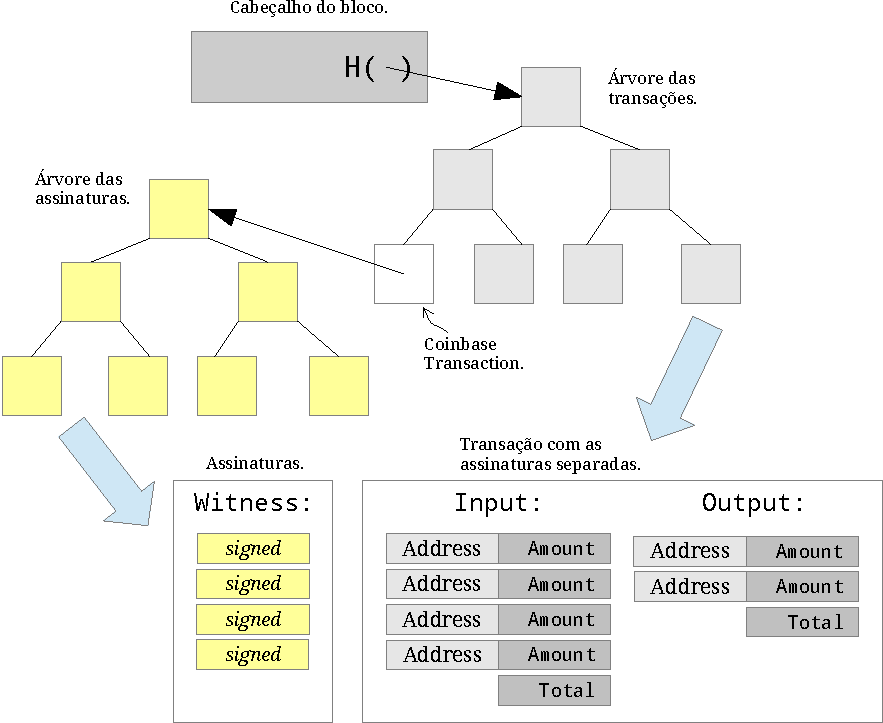
\includegraphics[scale=0.95]{./images/witness.pdf}
	\caption{Ilustração simplificada de um bloco cujas transações têm suas assinaturas separadas. \label{fig:witness}}
\end{figure}

Desde quando SegWit foi apresentado, ele tem tido um crescente suporte pela comunidade Bitcoin, pois possui baixo risco de implementação e adoção (\textbf{soft fork}), não interferindo nas regras de consenso.

\section{Lightning Network}

Lightning Network é uma grande inovação para a escalabilidade da blockchain. Essa proposta muda a maneira como vemos a blockchain hoje: a ideia é que ela funcione como um respaldo para canais de pagamentos entre usuários. Esses canais permitem que vários pagamentos sejam feitos fora da blockchain e somente o pagamento resultante é então propagado para a blockchain, representando o fechamento do canal \cite{bib:lightning-network}.

Para abrir um canal de pagamentos, é preciso uma transação que associe uma quantidade de bitcoins. Suponha que Alice deseja abrir um canal com Bob com a quantidade de 1 BTC. Para isso, ela cria uma transação multi-assinada por ela e por Bob pagando 1 BTC para um endereço dela e zero para um endereço de Bob. Tal transação é assinada por ambos e não é propagada para a blockchain. Tendo essa transação com respaldo, agora Alice pode criar novas transações atualizando o valor do pagamento, por exemplo, 0.9 BTC para ela e 0.1 BTC para Bob e novamente essa transação é assinada por ambos e não é propagada. Alice pode atualizar o valor do pagamento inúmeras vezes aumentando o valor para Bob e diminuindo para ela. Essas atualizações são vistas como micro-pagamentos e Bob tem o incentivo de propagar somente a última transação, pois é que lhe atribui maior valor. Ao propagar a última transação para a blockchain, esse canal de pagamentos é fechado.

Para assegurar que esse mecanismo funcione corretamente e também bidirecionalmente (Bob podendo criar transações atualizando os valores), é necessário, além das multi-assinaturas, a regra de \textit{nLockTime} que invalida uma transação após um período de tempo. Assim, a cada nova transação atualizando os valores, o \textit{nLockTime} é reduzido o que garante que a mais nova transação será aceita primeiro na blockchain se ela for propagada.

\begin{figure}[h!]
	\centering
	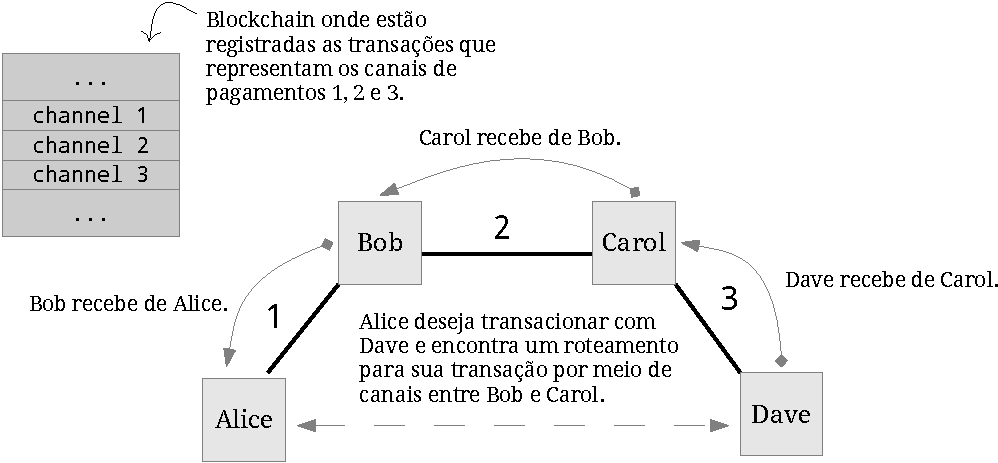
\includegraphics[scale=0.9]{./images/lightning-network.pdf}
	\caption[Ilustração simplificada de uma rede de canais de pagamentos.]{Ilustração simplificada de uma rede de canais de pagamentos. Alice deseja transacionar com Dave e para isso usa um roteamento possível por meio de Bob e Carol. Primeiramente, Dave recebe de Carol, depois Carol recebe de Bob e por fim Bob recebe de Alice. \label{fig:lightning-network}}
\end{figure}

\newpage
Indo além de micro-pagamentos entre dois usuários, a ideia da Lightning Network é compor uma rede inteira de canais de pagamentos em cima da rede Bitcoin. Para isso, os usuários mantém uma pequena quantidade de canais abertos durante longos períodos de tempo (semanas, meses ou até anos) formando uma rede por meio da qual é possível realizar roteamento de pagamentos entre usuários que não têm canal entre si (Figura~\ref{fig:lightning-network}). Para o correto funcionamento dessa rede, são propostos modelos criptográficos que asseguram a honestidade dos nós envolvidos no roteamento.

Por fim, uma vantagem implícita nessa inovação é o reforço contra regulamentações. Como a rede de canais de pagamentos aumenta a capacidade de pseudoanonimidade da rede --- perceba que a maioria das transações são vistas somente pelos envolvidos --- a dificuldade de regulamentar o Bitcoin aumenta.

\section{Considerações Finais}

O debate sobre escalabilidade é grande na comunidade Bitcoin. Foram aqui apresentadas as ideias principais de algumas das propostas recentemente discutidas. Espera-se por implementações confiáveis dessas ideias nos próximos anos, sendo SegWit a mais factível. Um outro fator que vem aumentando a necessidade por escalabilidade para uma maior adoção da moeda, é o \textit{reward halving} previsto para julho de 2016 em que a recompensa por bloco minerado reduzirá de 25 para 12,5 BTC.